\subsection{Domain-side Middleware}

%TODO For the sake of completeness, domain-side should also feature its own figure, now its strange to be less detailed than the client side. Otherwise, explicitly say at the start of the section that the domain side was only a demonstrative prototype [Martin]

The domain-side middleware prototype described herein focuses on a local-edge domain, and includes a complete realization of all four of A3-E's phases. It was implemented using Python\footnote{Documentation and source code are available at \url{https://github.com/deib-polimi/A3-E-DSM/}}, and is run on a Linux-based VM that hosts OpenWhisk\footnote{\url{http://openwhisk.incubator.apache.org/}}, a well-known open source FaaS platform. In particular, the prototype implements:

\begin{itemize}

	\item an advertisement mechanism that broadcasts UDP messages using a port that is known by the clients, with a frequency that is configurable (default $n=5$). A unicast channel is also created through which new clients should reply to the discovery of a domain using the address extracted from the advertisement broadcast. Once again the port is known in advance.

	\item an acquisition mechanism that downloads and installs (or upgrades existing) micro-services based on new application requirements. More precisely, the prototype receives a message from the client-side middleware containing the name of the required micro-service and its public source repository (e.g., git). After fetching the software artifacts from the repository, the acquisition mechanism searches for a service descriptor that specifies the function(s) that need to be (built and) allocated and additional artifacts. Lst.~\ref{lst:service-descriptor} illustrates the descriptor of an image recognition service with a single Java function and two dependencies used for image classification.

	\item an allocation mechanism that adds the acquired function(s) to OpenWhisk by means of its command-line API, and returns a message to the client-side middleware with the final name of the deployed micro-service along with the operation result. OpenWhisk places the function instances on its internal pool of containers, and creates an appropriate REST interface for the micro-service. Whilst the endpoint is mapped to a single function, the later may perform internal calls to other functions composing the micro-services.

\end{itemize}

\definecolor{lightgrey}{gray}{0.994}
\definecolor{blue}{rgb}{0, 0, 0.25}

\lstset{
	backgroundcolor=\color{lightgrey},
	basicstyle=\footnotesize\color{black},
    string=[s]{"}{"},
    stringstyle={\footnotesize\bfseries\color{blue}},
    comment=[l]{:},
    commentstyle={\footnotesize\color{black}},
    upquote=true,
    %numbers=left,
    %numbersep=5pt,
	%numberstyle=\tiny\color{black}    
}

\begin{minipage}{\linewidth}
\begin{lstlisting}[caption=Image recognition service descriptor, label=lst:service-descriptor, captionpos=t]
{
	"service-name":	"image-recognition",
	"functions": [{	
		"language":	"Java",
		"name":		"image-recognition",
		"source":	"it.polimi.a3e.imagerecognition.ImageRecognition",
		"build":	"true",
		"web":		"true"
		
	]
	"dependencies": ["NetSSD_deploy.prototxt", "NetSSD_deploy.caffemodel"]
}
\end{lstlisting}
\end{minipage}

%Martin's old server side details

%Figure~\ref{fig:reference-architecture} shows the proposed architecture for the compute continuum. Particular focus is put on the interaction between devices and Edge domain servers, since it is the main contribution of this paper. 
%The main physical elements are mobile devices and domain servers. Mobile devices can be of any type (e.g., tablets, smartphones), running several low-latency applications that needs offloading part of their computation to more powerful servers. For this, the devices send information to be processed to the domain server through standardized network protocols~\cite{Sill17standards}.  A Base Transceiver Station\footnote{Different generations of wireless mobile networks use distinct names (e.g., eNodeB in 4G).} (BTS) bridges mobile devices and domain servers as a part of the cellular infrastructure and  Edge architecture, according to its current specifications~\cite{hu2015mobile}. In this scenario, mobile devices and Edge domain servers are at no more than a few hops from each other. These servers host a serverless infrastructure, where stateless functions are deployed and executed according to the phases defined by the A3-E model. 
%The following sections provide details about the A3-E middleware (Section~\ref{subsec:A3-E}) and the serverless infrastructure that materializes Edge domain servers (Section~\ref{subsec:ServerlessArchCont}).
%
%\subsection{Edge-FaaS}
%\label{subsec:ServerlessArchCont}
%
%Following we briefly describe the serverless architecture that materializes the notion of Edge domains --- as shown in Figure~\ref{fig:domain-edge-arch}. 
%
%\begin{figure}[htb]
%	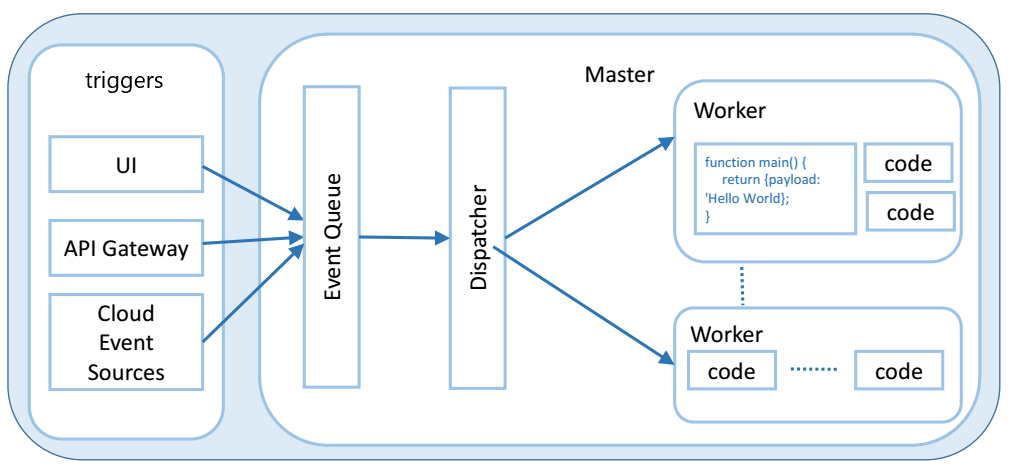
\includegraphics[width=.7\textwidth]{figs/ServerlessGenericArchEdit}
%	\caption{Serverless Architecture in the Domain Server}
%	\label{fig:domain-edge-arch}
%\end{figure}
%
%While Edge servers are ideal candidates for offloading the computation to preserve devices' battery life and reduce latency, these domain nodes are themselves potentially resource-constrained. Accordingly, the feasibility of hosting dedicated \textit{virtual machines}, \textit{containers}, and \textit{stateful applications} would also be limited, as these nodes cannot scale ``infinitely" to host always-running VMs/containers as the cloud itself. To overcome this limitation, we propose to materialize Edge domain servers through a serverless architecture~\cite{Roberts:2016,GarrigaMendonca2017}. 
%
%Figure~\ref{fig:domain-edge-arch} details the serverless components deployed on the domain server. The entry points are the \textit{triggers} associated with events --- e.g.,  mobile sensor readings or HTTP requests from mobile apps.  
%%in the MAR application, an event that triggers a function consists of uploading of an image or capturing a frame with the device's camera. --e.g., changes to database records, mobile sensor readings, code commits to a repository, or simple HTTP requests from Web or mobile apps. 
%These triggers fire requests to an \textit{Http Server} that exposes available functions as REST endpoints. 
%
%To achieve network transparency, a local Domain Name Server (DNS), deployed on the cellular infrastructure, must distinguish between requests addressed to the A3-E middleware/RESTful functions exposed by the domain server, and any other request for an Internet endpoint. The main difference from a regular DNS is locality, as the requests must be handled by the domain server on the current base station. To this end, the names of edge resources must be resolved locally without being propagated to public DNS servers. Whereas the specific details of the naming solution are outside the scope of this work, we argue that such a feature should not pose a significant technical challenge.% as it is already partially supported by the cellular infrastructure [CITE? is it right?].
%
%Once a request reaches the domain server, it is then forwarded to a \textit{controller} component, which identifies and retrieves the function being called, authorizes the execution of such a function and identifies an available invoker to run it. \textit{Invokers} isolate the \textit{functions} in containerized environments, optimized and managed by the serverless provider to reduce overhead and response time. Note that cold starts can happen when the controller allocates an inactive/new function for the first time. It increases time for the first call while the provider provisions the invoker (runtime container) and then runs the function. However, when the function is still allocated or warm --- since it was engaged recently by the same or a different client --- the environment stays alive, ready and waiting for execution. Eventually, after a period of inactivity (that depends on the size of the function and the current load of the server), the provider can drop the container and the function be deallocated, freeing resources for other functions.
%
%
%Finally, after execution, results and logging information are stored in the \textit{Storage} component, a highly available, noSQL database. Note that most of the components of the serverless architecture of the domain server are shared 
%%(in grey in Figure~\ref{fig:abstract_architecture}) 
%among all the functions. The highly shared nature and the automated management of the whole platform allows any function allocated on the domain servers to scale up automatically and elastically to unexpected bursts in the workload, and to scale down when it is not used anymore. In contrast with container-based stateful applications, the serverless platform is responsible for allocating functions of one or more applications on a pool of shared containers, according to the resources available at the domain server. As a result, the use of the computational resources of domain servers is optimized, allowing both more functions to be deployed and more requests to be processed simultaneously.
%
%Needless to say, an IaaS/FaaS cloud domain can always be selected to allocate and engage functions when required --- due to unavailability/overload of edge domain servers. Their implementation is similar to those described above, although details can vary among different vendors\footnote{\url{https://github.com/apache/incubator-openwhisk/blob/master/docs/about.md}}.
%
%As an advantage over the traditional, ``serverful'' approaches, it is not necessary to pre-allocate multiple virtual machines or containers to be resilient and responsive against downtime of single instances or bursts of workload. The on-demand execution of functions provides inherent scalability and optimal utilization as the number of running functions always matches the trigger rate. Additionally, the application developer only focuses on the application code and can fully outsource the management of the execution infrastructure to the A3-E middleware. The serverless approach also provides a fine-grained \textit{pay-per-use} billing model with benefits for both application owners and telecom operators (in charge of the domain servers).